\documentclass[10pt,a4paper]{report}
\usepackage[utf8]{inputenc}
\usepackage[english]{babel}
\usepackage{amsmath}
\usepackage{amsfonts}
\usepackage{amssymb}
\usepackage{graphicx}
\usepackage[left=2cm,right=2cm,top=2cm,bottom=2cm]{geometry}
\usepackage[autostyle, italian=quotes]{csquotes}
\usepackage{hyperref}
\author{Daniele Gilio}
\title{Exam Assignment}
\begin{document}
\maketitle
\section{Introduction}
This assignment was about text classification. We had to classify News titles by their topic; our classes were \enquote{science}, \enquote{health}, \enquote{business} and \enquote{entertainment}. Our raw features were the title itself and the publisher. The dataset was already divided in $10000$ training samples, $1000$ validation samples and $1000$ test samples. Our objective is to create a feature extraction process and to build one or more classifiers.
\section{Feature Extraction}
Since we are dealing with text classification we chose to employ the Bag of Words representation to encode the titles. In order to do that we had to build a fixed size dictionary. In Figure \ref{fig:acc_vs_dic} we can see how the dictionary size affects the performance of the models we intend to build.
\begin{figure}[!ht]
\centering
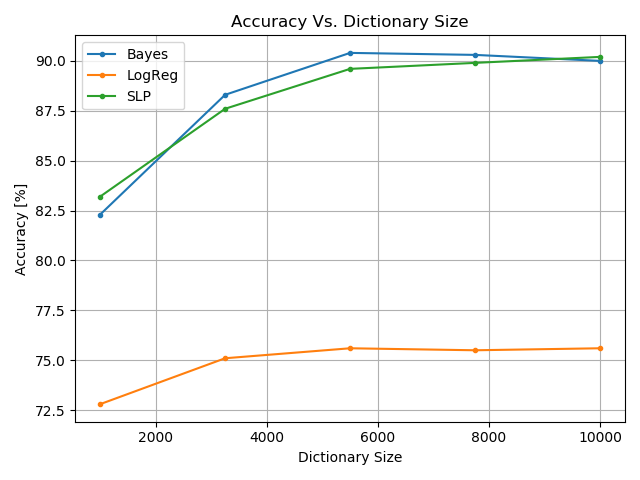
\includegraphics[width=0.5\linewidth]{acc_vs_dic.png}
\caption{Test Accuracy vs. Dictionary Size}
\label{fig:acc_vs_dic}
\end{figure}
Our goal with Figure \ref{fig:acc_vs_dic} was not to find the optimal dictionary size but to see if a bigger dictionary implied a better performance and this seems to be the case. Another decision we had to make was choosing if the publisher was a useful feature to keep. 
\begin{figure}[!ht]
\centering
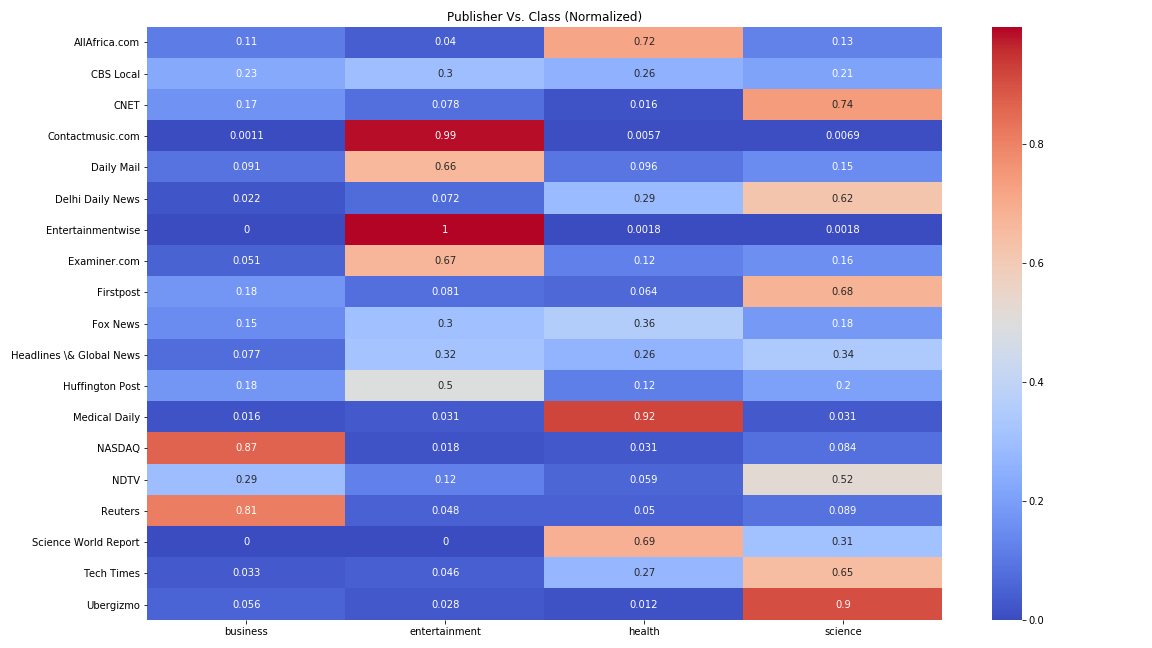
\includegraphics[width=0.75\linewidth]{pub_vs_class.png}
\caption{Publisher Class Distribution}
\label{fig:pub_vs_class}
\end{figure}
As we can see from Figure \ref{fig:pub_vs_class}, the $19$ different publishers mostly belong to a couple of classes. Based on that information we decide to keep the publisher information and we concatenated it to the title BoW. The simplest solution we found to encode the publishers was just to number them from $0$ to $18$. We also took into consideration normalization techniques, both in terms of words normalization (remove common words from the dictionary and stemming) and BoW normalization. We found out that using only one word normalization technique worsened the performance of all the models but using them both made them perform better. That said we used word normalization techniques for all the test we performed. Each model reacted differently to different BoW normalizations so we will discuss them separately.  
\section{Classifiers}
We decided to build a total of $4$ classifiers: Multinomial Bayesian Classifier, Multinomial Logistic Regression, Single Layer Perceptron and Multi-Layer Perceptron. The first two choices were biased upon the results we obtained in the Sentiment Analysis assignment. The latter two were chosen because of their versatility and previous assignments results. To be completely honest we would have liked to use SVMs since they proved to be the best in text recognition but we cannot since we are dealing with a multi-class problem, we would need a sort of multinomial SVM for which we do not have the theoretical background nor any code ready to be used. We settled on a dictionary size of $8000$ words, as it is very close to the maximum possible size given the normalizations performed on the corpus.
\subsection{Multinomial Naive Bayesian Classifier}
We chose the \textit{Multinomial Bayesian Classifier} as our baseline for testing since it proved to be simple but effective. Its simplicity meant that we could run multiple tests without worrying about the computational time needed to train it. The results of this classifier caught us off guard and proved to be challenging to beat. The Multinomial Bayesian Classifier reacted poorly upon BoW Normalization. L1 and L2 nearly cut the test accuracy in half and MaxAbs lowered it by a couple of percentage points. With those results we chose not to use any normalization to let this classifier perform at its best. The training accuracy was $94.39 \%$, the validation one was $89.2 \%$ and the test one was $91.1 \%$.
\begin{figure}[!ht]
\centering
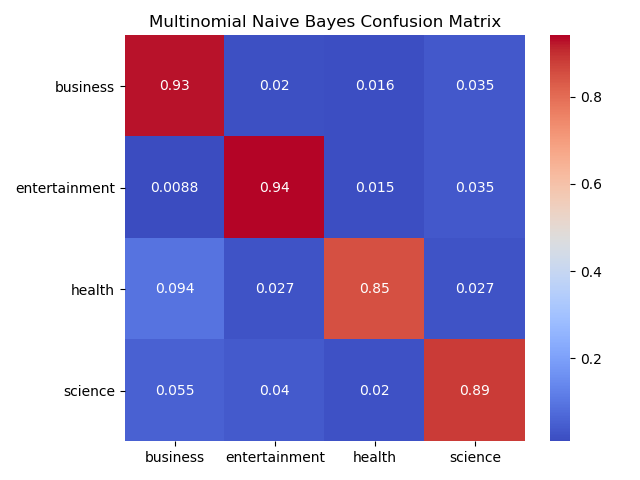
\includegraphics[width=0.5\linewidth]{bayes_confmat.png}
\caption{Bayesian Classifier Confusion Matrix (Test Set)}
\label{fig:bayes_confmat}
\end{figure}
\subsection{Multinomial Logistic Regression}
The \textit{Multinomial Logistic Regression} classifier was the most disappointing amongst all the classifiers we tested. Not only did it perform quite terribly if compared to the others but it also took a very long time to train (even if we used a version that leverages a CUDA GPU). We used a constant learning rate ($\gamma=10^{-2}$) since a test with a variable one did produce worse results. A lower learning rate also worsened the results. We set the normalization constant at $\lambda=10^{-5}$ and we trained it for $10000$ steps. This model reacted to BoW normalization as the Bayesian Classifier so we did not apply any. 
\subsection{Single Layer Perceptron}
\subsection{Multi-Layer Perceptron}
\section{Results Analysis}
\section{Conclusions}
\end{document}